\documentclass[border=0pt]{standalone}
\usepackage{amsmath,amssymb}
\usepackage{lmodern}
\usepackage[default,semibold]{sourcesanspro}
\usepackage[scale=0.92]{sourcecodepro}
\usepackage{fontawesome5}
\usepackage{tikz}
\usetikzlibrary{arrows.meta,calc,positioning,backgrounds,fit,decorations.pathreplacing}
\pgfdeclarelayer{edges}
\pgfsetlayers{background,edges,main}

\definecolor{brand}{HTML}{6A3DF0}
\definecolor{brandlight}{HTML}{A78BFA}
\definecolor{lavender}{HTML}{F4F0FF}
\definecolor{ink}{HTML}{151A2D}
\definecolor{muted}{HTML}{6B6B80}
\definecolor{hairline}{HTML}{E8E5F0}
\definecolor{qloo}{HTML}{14B8A6}
\definecolor{qloodark}{HTML}{0F766E}
\definecolor{qlootint}{HTML}{ECFAF8}
\definecolor{llm}{HTML}{9CA3AF}
\definecolor{llmdark}{HTML}{6B7280}
\definecolor{llmtint}{HTML}{F6F7F9}

\newcommand{\fsHead}{\fontsize{11}{13}\selectfont}
\newcommand{\fsTitle}{\fontsize{9.5}{11.5}\selectfont}
\newcommand{\fsBody}{\fontsize{8.5}{10.5}\selectfont}
\newcommand{\fsSmall}{\fontsize{7.5}{9.2}\selectfont}
\newcommand{\fsTiny}{\fontsize{7}{8.4}\selectfont}
\newcommand{\kicker}[1]{{\fontsize{7.5}{9}\selectfont\bfseries\addfontfeature{LetterSpace=9}\MakeUppercase{#1}}}
\newcommand{\code}[1]{{\ttfamily #1}}
\newcommand{\tokens}[1]{{\fsTiny\bfseries #1}}
\newcommand{\rarr}{{\color{brand}$\rightarrow$}\ }
\newcommand{\larr}{{\color{brand}$\leftarrow$}\ }
\newcommand{\sto}{$\rightarrow$}

\tikzset{
  figure/.style={
    show background rectangle,
    inner frame sep=14pt,
    background rectangle/.style={fill=white, draw=none},
    font=\fsBody, text=ink, line cap=round, line join=round,
  },
  card/.style={
    rounded corners=6pt, draw=hairline, line width=0.8pt, fill=white,
    align=center, inner sep=5pt, text=ink,
  },
  zone/.style={
    rounded corners=12pt, draw=brandlight!55, line width=0.8pt, fill=lavender,
  },
  chip/.style={
    rounded corners=4pt, fill=lavender, draw=none, text=brand,
    font=\fsSmall, inner xsep=5pt, inner ysep=3pt, align=center,
  },
  qloocard/.style={card, draw=qloo, fill=qlootint},
  llmcard/.style={card, draw=llm, fill=llmtint, dash pattern=on 3pt off 2pt},
  arrow/.style={
    draw=ink!65, line width=0.9pt,
    -{Stealth[length=6pt, width=4.6pt, round]},
  },
  twoway/.style={
    draw=ink!65, line width=0.9pt,
    {Stealth[length=6pt, width=4.6pt, round]}-{Stealth[length=6pt, width=4.6pt, round]},
  },
  lbl/.style={font=\fsTiny, text=muted, align=center, inner sep=1.5pt},
  badge/.style={
    rounded corners=5pt, font=\fsTiny\bfseries, inner xsep=4pt, inner ysep=2pt,
    fill=lavender, text=brand,
  },
}


\tikzset{
  tag/.style={rounded corners=5pt, font=\fsTiny\bfseries, inner xsep=5pt, inner ysep=2.5pt},
  tagdev/.style={tag, fill=white, text=brand, draw=brandlight, line width=0.7pt},
  tagnode/.style={tag, fill=brand, text=white},
  tagqloo/.style={tag, fill=qloo, text=white},
  tagllm/.style={tag, fill=llm, text=white},
  taggraph/.style={tag, fill=white, text=brand, draw=brand, line width=0.6pt},
  free/.style={badge},
  paid/.style={badge, fill=white, text=llmdark, draw=llm, line width=0.6pt},
  stage/.style={card, minimum height=4.0cm, anchor=south west},
  body/.style={align=flush center, inner sep=0pt, anchor=north},
}

\newcommand{\devtag}{\faLaptop\ device}
\newcommand{\nodetag}{\faServer\ PCP node}

\begin{document}
\begin{tikzpicture}[figure]

\node[stage, minimum width=1.95cm] (c1) at (0,0.6) {};
\node[stage, minimum width=2.1cm] (c2) at (2.37,0.6) {};
\node[stage, minimum width=2.55cm] (c3) at (4.89,0.6) {};
\node[stage, minimum width=2.2cm, draw=qloo, fill=qlootint] (c4) at (7.86,0.6) {};
\node[stage, minimum width=2.2cm] (c5) at (10.48,0.6) {};
\node[stage, minimum width=2.25cm, draw=brandlight, fill=lavender] (c6) at (13.1,0.6) {};
\node[stage, minimum width=1.95cm] (c7) at (15.77,0.6) {};

\foreach \a/\b in {c1/c2, c2/c3, c3/c4, c4/c5, c5/c6, c6/c7} {
  \draw[arrow, draw=brand] (\a.east) -- (\b.west);
}

\node[tagdev] at (c1.north) {\devtag};
\node[body] at ($(c1.north)+(0,-0.38)$)
  {{\fsTitle\bfseries Request}\\[6pt]{\fsSmall\itshape ``Something}\\{\fsSmall\itshape to watch on}\\{\fsSmall\itshape Friday night''}\\[6pt]{\fsTiny\color{muted}+ public names}\\{\fsTiny\color{muted}+ 3 weights}};

\node[tagnode] at (c2.north) {\nodetag};
\node[body] at ($(c2.north)+(0,-0.38)$)
  {{\fsTitle\bfseries Type}\\[2pt]{\fsSmall\color{brand}Naive Bayes}\\[5pt]{\fsTiny\color{muted}on the task words}\\{\fsTiny\color{muted}(learned counts)}};
\node[chip, font=\fsTiny] at ($(c2.south)+(0,1.75)$) {\textbf{movie} \textperiodcentered\ 0.81};
\node[free] at ($(c2.south)+(0,0.4)$) {0 LLM tokens};

\node[body] at ($(c3.north)+(0,-0.18)$) {{\fsTitle\bfseries Candidates}};
\draw[llmcard] ($(c3.south west)+(0.13,2.12)$) rectangle ($(c3.south east)+(-0.13,3.2)$);
\node[tagllm] at ($(c3.south)+(0,3.2)$) {LLM agent};
\node[font=\fsTiny, text=muted] at ($(c3.south)+(0,2.83)$) {8 picks + priors};
\node[paid] at ($(c3.south)+(0,2.4)$) {1 LLM call};
\node[font=\fsTiny\bfseries, text=muted] at ($(c3.south)+(0,1.93)$) {or};
\draw[card, draw=brandlight] ($(c3.south west)+(0.13,0.15)$) rectangle ($(c3.south east)+(-0.13,1.6)$);
\node[taggraph] at ($(c3.south)+(0,1.6)$) {graph-only};
\node[body, font=\fsTiny, text=muted] at ($(c3.south)+(0,1.33)$) {\code{qloo\_recommend}\\+ PC graph picks};
\node[free] at ($(c3.south)+(0,0.4)$) {0 LLM tokens};

\node[tagqloo] at (c4.north) {Qloo};
\node[body] at ($(c4.north)+(0,-0.38)$)
  {{\fsTitle\bfseries Affinity}\\[2pt]{\fsSmall\color{qloodark}\code{qloo\_rank}}\\[5pt]{\fsTiny\color{muted}every option vs.}\\{\fsTiny\color{muted}your favorites}\\[5pt]{\fsTiny\color{qloodark}graph-only: from}\\{\fsTiny\color{qloodark}\code{qloo\_recommend}}};
\node[free, fill=white] at ($(c4.south)+(0,0.4)$) {0 LLM tokens};

\node[tagnode] at (c5.north) {\nodetag};
\node[body] at ($(c5.north)+(0,-0.38)$)
  {{\fsTitle\bfseries Graph score}\\[2pt]{\fsSmall\color{brand}Personalized}\\{\fsSmall\color{brand}PageRank}\\[5pt]{\fsTiny\color{muted}adds qloo edges,}\\{\fsTiny\color{muted}seeds at You}\\{\fsTiny\color{muted}$\alpha=0.15$}};
\node[free] at ($(c5.south)+(0,0.4)$) {0 LLM tokens};

\node[tagdev] at (c6.north) {\devtag};
\node[body] at ($(c6.north)+(0,-0.38)$)
  {{\fsTitle\bfseries Re-weight}\\[2pt]{\fsSmall\color{brand}conditional logit}\\[6pt]{\fsSmall$p_i\propto\exp(\mathbf{w}^{\top}\mathbf{x}_i)$}\\[6pt]{\fsTiny\color{muted}agent prior, Qloo}\\{\fsTiny\color{muted}affinity, graph score}};
\node[free, fill=white] at ($(c6.south)+(0,0.4)$) {0 LLM tokens};

\node[tagdev] at (c7.north) {\devtag};
\node[body] at ($(c7.north)+(0,-0.38)$)
  {{\fsTitle\bfseries Answer}\\[6pt]{\fsTiny\color{muted}ranked picks}\\{\fsTiny\color{muted}with Qloo and}\\{\fsTiny\color{muted}graph provenance}};
\node[free] at ($(c7.south)+(0,0.4)$) {0 LLM tokens};

\draw[line width=1pt, draw=brand, rounded corners=8pt] (c7.south) -- ($(c7.south)+(0,-1.0)$) -- ($(c2.south)+(0,-1.0)$) -- ($(c2.south)+(0,-0.3)$);
\draw[arrow, draw=brand] ($(c2.south)+(0,-0.35)$) -- (c2.south);
\draw[arrow, draw=brand] ($(c6.south)+(0,-1.0)$) -- (c6.south);
\draw[arrow, draw=brand] ($(c5.south)+(0,-1.0)$) -- (c5.south);
\fill[brand] ($(c6.south)+(0,-1.0)$) circle (1.7pt) ($(c5.south)+(0,-1.0)$) circle (1.7pt);
\node[fill=white, text=brand, inner sep=2pt, font=\fontsize{9}{9}\selectfont] at ($(c7.south)+(0,-0.45)$) {\faThumbsUp\,\faThumbsDown[regular]};
\node[lbl, anchor=east] at ($(c7.south)+(-0.42,-0.45)$) {like / dislike};

\node[lbl, anchor=north] at ($(c2.south)+(0,-1.12)$) {{\bfseries\color{brand}type counts}\\learn the task words (on like)};
\node[lbl, anchor=north] at ($(c5.south)+(0,-1.12)$) {{\bfseries\color{brand}PC graph edges}\\like, co-liked, veto};
\node[lbl, anchor=north] at ($(c6.south)+(0.35,-1.12)$) {{\bfseries\color{brand}weights on device}\\$\mathbf{w}\leftarrow\mathbf{w}\pm\eta\,(\mathbf{x}_c-\mathbb{E}_p[\mathbf{x}])$};
\node[free, fill=white, draw=brandlight, line width=0.5pt] at ($(c3.south)+(1.3,-1.0)$) {feedback: 0 LLM tokens};

\node[anchor=north west, align=left, font=\fsSmall, text=muted, inner sep=0pt] at (0,-1.42)
  {\textbf{\color{ink}Per request:} one LLM call with an agent, \textbf{\color{brand}0 LLM tokens} in graph-only mode. Every other step is classical.};

\end{tikzpicture}
\end{document}
